% =====================================================================
%  KARIOS CubeSat -- Model-Based Systems Engineering (MBSE) Process
%  Schematic block diagram
%
%  Grounded in:
%   * draft_mikael.pdf  (KAIST Intelligence & Reconnaissance Orbital Satellite)
%   * INCOSE SSWG CubeSat Reference Model (CRM) -- Kaslow et al. (RAX mission)
%   * Developing a CubeSat MBSE Reference Model (Interim status)
%
%  Compile:  pdflatex KARIOS_mbse_block_diagram.tex
% =====================================================================
\documentclass[border=14pt]{standalone}
\usepackage[T1]{fontenc}
\usepackage{helvet}
\renewcommand{\familydefault}{\sfdefault}
\usepackage{tikz}
\usetikzlibrary{positioning,arrows.meta,fit,backgrounds,calc}

% ---- palette ----
\definecolor{accent}{HTML}{2563A8}
\definecolor{ink}{HTML}{131B28}
\definecolor{ink3}{HTML}{6B7788}
\definecolor{line}{HTML}{C4CDD9}
\definecolor{surface}{HTML}{FFFFFF}
\definecolor{surface2}{HTML}{F1F4F9}
\definecolor{creq}{HTML}{2F74C0}   % Requirements
\definecolor{cstr}{HTML}{1F8F86}   % Structure
\definecolor{cbeh}{HTML}{7C53A5}   % Behavior
\definecolor{cpar}{HTML}{C9761F}   % Parametrics
\definecolor{warn}{HTML}{C0632A}

\begin{document}
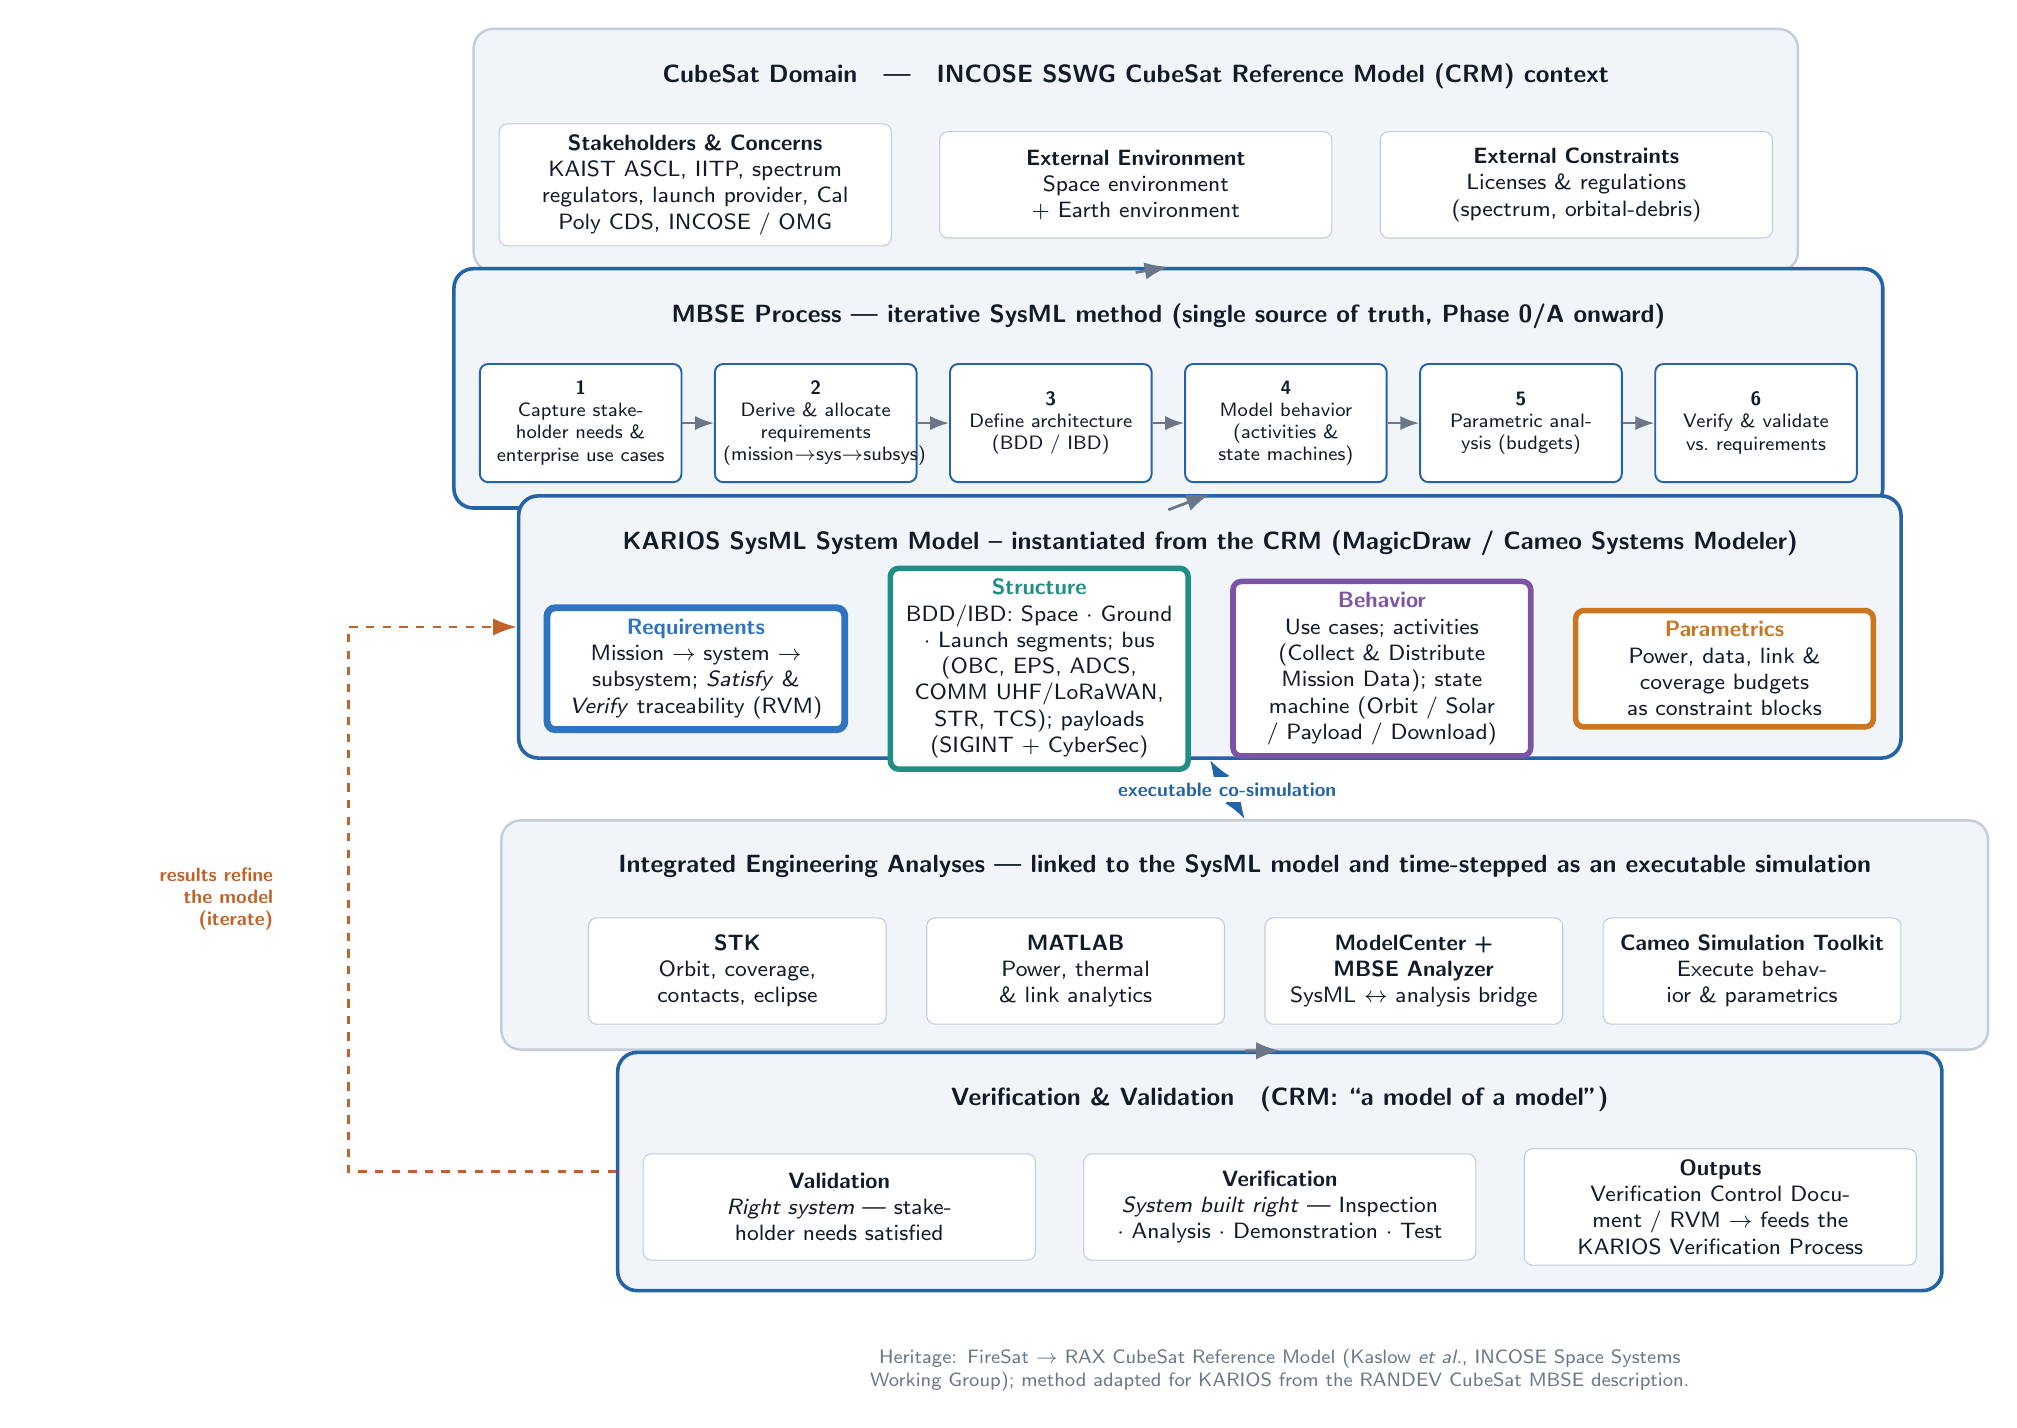
\begin{tikzpicture}[
  font=\small,
  every node/.style={text=ink},
  chip/.style={draw=line, rounded corners=3pt, fill=surface, align=center,
               inner sep=4pt, font=\footnotesize, text width=3.5cm, minimum height=1.35cm},
  pstep/.style={draw=accent, rounded corners=3pt, fill=surface, align=center,
               inner sep=3pt, font=\scriptsize, text width=2.35cm, minimum height=1.5cm, line width=0.7pt},
  gtitle/.style={font=\bfseries\small, text=ink, align=center},
  group/.style={draw=line, line width=0.9pt, rounded corners=7pt, fill=surface2, inner sep=9pt},
  keygroup/.style={group, draw=accent, line width=1.3pt},
  down/.style={-{Latex[length=3mm,width=2.2mm]}, line width=1pt, draw=ink3},
  bidir/.style={{Latex[length=3mm]}-{Latex[length=3mm]}, line width=1pt, draw=accent, dashed},
  rarrow/.style={-{Latex[length=2.4mm]}, line width=0.8pt, draw=ink3},
]

% ================= BAND 1 : CUBESAT DOMAIN (context) =================
\node[chip, text width=4.7cm] (x1)
   {\textbf{Stakeholders \& Concerns}\\ KAIST ASCL, IITP, spectrum regulators, launch provider, Cal Poly CDS, INCOSE / OMG};
\node[chip, text width=4.7cm, right=6mm of x1] (x2)
   {\textbf{External Environment}\\ Space environment + Earth environment};
\node[chip, text width=4.7cm, right=6mm of x2] (x3)
   {\textbf{External Constraints}\\ Licenses \& regulations (spectrum, orbital-debris)};
\node[gtitle] (xttl) at ([yshift=6.5mm]$(x1.north)!0.5!(x3.north)$)
   {CubeSat Domain \; --- \; INCOSE SSWG CubeSat Reference Model (CRM) context};
\begin{scope}[on background layer]
  \node[group, fit=(xttl)(x1)(x3)] (ctxbox) {};
\end{scope}

% ================= BAND 2 : MBSE PROCESS SPINE =================
\node[pstep,below=1.15cm of ctxbox.south, xshift=-7.05cm] (s1)
   {\textbf{1}\\ Capture stakeholder needs \& enterprise use cases};
\node[pstep,right=4mm of s1] (s2) {\textbf{2}\\ Derive \& allocate requirements (mission$\to$sys$\to$subsys)};
\node[pstep,right=4mm of s2] (s3) {\textbf{3}\\ Define architecture (BDD / IBD)};
\node[pstep,right=4mm of s3] (s4) {\textbf{4}\\ Model behavior (activities \& state machines)};
\node[pstep,right=4mm of s4] (s5) {\textbf{5}\\ Parametric analysis (budgets)};
\node[pstep,right=4mm of s5] (s6) {\textbf{6}\\ Verify \& validate vs.\ requirements};
\foreach \a/\b in {s1/s2,s2/s3,s3/s4,s4/s5,s5/s6}{ \draw[rarrow] (\a) -- (\b); }
\node[gtitle] (sttl) at ([yshift=6mm]$(s1.north)!0.5!(s6.north)$)
   {MBSE Process --- iterative SysML method (single source of truth, Phase 0/A onward)};
\begin{scope}[on background layer]
  \node[keygroup, fit=(sttl)(s1)(s6)] (spinebox) {};
\end{scope}

% ================= BAND 3 : KARIOS SysML MODEL (4 pillars) =================
\node[chip, draw=creq, line width=2.5pt, below=1.2cm of spinebox.south, xshift=-6.0cm] (p1)
   {\textbf{\textcolor{creq}{Requirements}}\\ Mission $\to$ system $\to$ subsystem; \emph{Satisfy} \& \emph{Verify} traceability (RVM)};
\node[chip, draw=cstr, line width=2pt, right=5mm of p1] (p2)
   {\textbf{\textcolor{cstr}{Structure}}\\ BDD/IBD: Space $\cdot$ Ground $\cdot$ Launch segments; bus (OBC, EPS, ADCS, COMM UHF/LoRaWAN, STR, TCS); payloads (SIGINT + CyberSec)};
\node[chip, draw=cbeh, line width=2pt, right=5mm of p2] (p3)
   {\textbf{\textcolor{cbeh}{Behavior}}\\ Use cases; activities (Collect \& Distribute Mission Data); state machine (Orbit / Solar / Payload / Download)};
\node[chip, draw=cpar, line width=2pt, right=5mm of p3] (p4)
   {\textbf{\textcolor{cpar}{Parametrics}}\\ Power, data, link \& coverage budgets as constraint blocks};
\node[gtitle, text width=16.5cm] (mttl) at ([yshift=8mm]$(p1.north)!0.5!(p4.north)$)
   {KARIOS SysML System Model -- instantiated from the CRM (MagicDraw / Cameo Systems Modeler)};
\begin{scope}[on background layer]
  \node[keygroup, fit=(mttl)(p1)(p4)] (modelbox) {};
\end{scope}

% ================= BAND 4 : INTEGRATED ANALYSES (tools) =================
\node[chip, below=2.0cm of modelbox.south, xshift=-6.0cm] (t1)
   {\textbf{STK}\\ Orbit, coverage, contacts, eclipse};
\node[chip, right=5mm of t1] (t2) {\textbf{MATLAB}\\ Power, thermal \& link analytics};
\node[chip, right=5mm of t2] (t3) {\textbf{ModelCenter + MBSE Analyzer}\\ SysML $\leftrightarrow$ analysis bridge};
\node[chip, right=5mm of t3] (t4) {\textbf{Cameo Simulation Toolkit}\\ Execute behavior \& parametrics};
\node[gtitle, text width=18cm] (tttl) at ([yshift=6.5mm]$(t1.north)!0.5!(t4.north)$)
   {Integrated Engineering Analyses --- linked to the SysML model and time-stepped as an executable simulation};
\begin{scope}[on background layer]
  \node[group, fit=(tttl)(t1)(t4)] (toolbox) {};
\end{scope}

% ================= BAND 5 : VERIFICATION & VALIDATION =================
\node[chip, text width=4.7cm, below=1.3cm of toolbox.south, xshift=-5.15cm] (v1)
   {\textbf{Validation}\\ \emph{Right system} --- stakeholder needs satisfied};
\node[chip, text width=4.7cm, right=6mm of v1] (v2)
   {\textbf{Verification}\\ \emph{System built right} --- Inspection $\cdot$ Analysis $\cdot$ Demonstration $\cdot$ Test};
\node[chip, text width=4.7cm, right=6mm of v2] (v3)
   {\textbf{Outputs}\\ Verification Control Document / RVM $\to$ feeds the KARIOS Verification Process};
\node[gtitle] (vttl) at ([yshift=6.5mm]$(v1.north)!0.5!(v3.north)$)
   {Verification \& Validation \; (CRM: ``a model of a model'')};
\begin{scope}[on background layer]
  \node[keygroup, fit=(vttl)(v1)(v3)] (vvbox) {};
\end{scope}

% ================= vertical connectors =================
\draw[down] (ctxbox.south)  -- (spinebox.north);
\draw[down] (spinebox.south) -- (modelbox.north);
\draw[bidir] (modelbox.south) -- node[fill=surface, inner sep=2pt, font=\scriptsize\bfseries, text=accent]
      {executable co-simulation} (toolbox.north);
\draw[down] (toolbox.south) -- (vvbox.north);

% feedback loop : V&V results refine the model (orthogonal: left -> up -> right)
\draw[down, draw=warn, dashed]
   (vvbox.west) -- ++(-3.4,0) |- (modelbox.west);
\node[anchor=east, text width=3cm, align=right, font=\scriptsize\bfseries, text=warn]
   at ([xshift=-3.6cm]$(vvbox.west)!0.5!(modelbox.west)$)
   {results refine\\ the model\\ (iterate)};

% ================= heritage caption =================
\node[font=\scriptsize, text=ink3, text width=17cm, align=center, below=6mm of vvbox.south]
   {Heritage: FireSat $\to$ RAX CubeSat Reference Model (Kaslow \emph{et al.}, INCOSE Space Systems Working Group); method adapted for KARIOS from the RANDEV CubeSat MBSE description.};

\end{tikzpicture}
\end{document}
